\documentclass[a4paper,12pt]{article}
\usepackage[T1,T2A]{fontenc}
\usepackage[utf8]{inputenc}
\usepackage[english,main=russian]{babel}

\usepackage[backend=biber,style=gost-numeric,sorting=none]{biblatex}
\addbibresource{bibliography.bib}
\renewcommand*{\bibfont}{\small}

\usepackage{listings}

\usepackage{polyglossia} %% загружает пакет многоязыковой вёрстки
\usepackage{csquotes}
\setdefaultlanguage{russian}
\setotherlanguage{english} %% объявляет второй язык документа
\defaultfontfeatures{Ligatures={TeX}}
% Times New Roman
\setromanfont[
BoldFont=Times New Roman Bold.ttf,
ItalicFont=Times New Roman Italic.ttf,
BoldItalicFont=Times New Roman Bold Italic.ttf,
]{Times New Roman.ttf}

\usepackage[labelsep={period}]{caption} % точка в подписях рисунков

\usepackage{sectsty}
\sectionfont{\fontsize{12}{15}\selectfont\MakeUppercase} % делает 12pt и апперкейс шрифтам в заголовках

\usepackage{graphicx} % рисунки
\graphicspath{ {figures/} }

\usepackage{wasysym} % спецсимволы для таблицы

\usepackage{hyperref} % гиперссылки

\usepackage{hyphenat} % переносы слов
\hyphenation{ма-те-ма-ти-ка вос-ста-нав-ли-вать}

\usepackage{indentfirst} % отделять первую строку раздела абзацным отступом тоже

\renewcommand{\labelitemi}{\textendash} % тире в списках

\linespread{1.3} % полуторный интервал

\usepackage{geometry} % поля страниц
\geometry{left=2cm}
\geometry{right=2cm}
\geometry{top=2.5cm}
\geometry{bottom=2.5cm}

\begin{document}

{\setlength{\parindent}{0cm}
УДК 004.5

\textbf{Матвей Михайлович Правосудов}, студент, e-mail: \href{mailto:matvey@pravosudov.com}{matvey@pravosudov.com}, 

Национальный исследовательский Томский политехнический университет,

\textbf{Игорь Петрович Скирневский}, ассистент, e-mail: \href{mailto:skirnevskiy@tpu.ru}{skirnevskiy@tpu.ru}
}

\begin{center}
\textbf{\MakeUppercase{Информационная система для анализа}}

\textbf{\MakeUppercase{слов русского языка «Словолит»}}
\end{center}

\textbf{Аннотация.} В статье освещается сервис для автоматического морфологического и морфемного анализа. Дополнительными функциями системы являются подбор синонимов и поиск значений слов русского языка. На данный момент существует ограниченный набор систем, позволяющих выполнять подобный анализ, а большинство алгоритмов нет в открытом доступе. Эти алгоритмы востребованы в сфере школьного образования. В основе логики работы системы лежат оцифрованные словари разборов Тихонова и Ефремовой. Для морфемного анализа разработан новый алгоритм на основе сравнения морфов в слове с морфемами из словаря. Система разработана на веб-стеке технологий, что позволяет использовать ресурс на любом устройстве, включая мобильный телефон или настольный браузер. Основным ограничением системы является отсутствие полного покрытия слов, так как язык постоянно расширяется и изменяется.

\textbf{Ключевые слова:} веб-сервис, морфологический анализ, морфемный анализ, значения слов, русский язык, автоматическая обработка текста.\\

{\setlength{\parindent}{0cm}
\textbf{Matvey Mikhailovich Pravosudov}, student, e-mail: \href{mailto:matvey@pravosudov.com}{matvey@pravosudov.com}, 

National Research Tomsk Polytechnic University,

\textbf{Igor Petrovich Skirnevskiy}, research engineer, e-mail: \href{mailto:skirnevskiy@tpu.ru}{skirnevskiy@tpu.ru}
}

\begin{center}
\textbf{\MakeUppercase{Informational system for analysis}}

\textbf{\MakeUppercase{of Russian language words called «Slovolit»}}
\end{center}

\textbf{Annotation.} The present study aimed to show a service for automatic morphological, morphemic and meaning analysis. Today there is a limited set of systems provided the same functionality. Moreover, and most algorithms are not available for public access. The presented system could be used for school education or professional linguists conducting linguistic research. A new algorithm has been developed for morphemic analysis. The algorithm uses Tikhonov’s and Efremova’s dictionaries to detect morphemic structure of a word. The main idea of the algorithm is comparing morphs in a word with morphemes from a dictionary. The system was developed on a web-based platform and can be used on any device including a mobile phone. The main drawback of the software is limitation of language dictionaries.

\textbf{Keywords:} web-service, morphological analysis, morphemic analysis, word meaning, Russian language, automatic text processing.

\newpage

\section*{Введение}
Русский язык – один из самых сложных для изучения языков. В нем достаточно много правил, но еще больше исключений. Существует ряд инструментов, помогающих людям изучать язык: словари, справочники и учебники. В силу развития технологий появилась масса сервисов в интернете, позволяющих, например, находить значения слов или производить какой-либо анализ. Основных разборов (анализов) несколько:
\begin{itemize}
\item Морфологический – разбор слова по частям речи, определение морфологического состава, с последующей характеристикой отдельных слов, относящихся к той или иной части речи.
\item Морфемный (структурный) – определение состава слова, например, приставки, корня, суффиксов и т. д.
\item Фонетический – анализ слоговой структуры и звукового состава слова.
\item Этимологический – определение происхождения слова.
\end{itemize}

Обычно сервисы по анализу слов работают не в одной «экосистеме», а раздробленно: каждый компонент ничего не знают о другом и работает независимо. Данное ограничение затрудняет комплексный анализ слов.

В данной статье описывается веб-сервис, позволяющий использовать унифицированный интерфейс для комплексного анализа нескольких слов. Главная часть интерфейса — командная строка запросов. Она поддерживает как ввод простого слова, так и расширение функционала при помощи вспомогательных синтаксических конструкций. Кроме того, интерфейс веб-сайта был разработан адаптивным, что позволяет легко использовать его на мобильных устройствах.

Такой сервис может быть использован как учащимися школ в качестве заменителя бумажных справочников, так и учителями русского языка и литературы для быстрого уточнения результатов разборов слов. Студенты и научные сотрдуники в сфере филологических наук смогут экономить время на обращении к бумажому словарю, благодаря быстрой работе сервиса. В силу того, что представленный веб-сервис адаптирован под мобильные устройства, его использование будет удобнее, нежели поиск разборов в нескольких книгах.

Веб-сервис является кросс-платформенным решением, позволяющим использовать его где угодно при наличии интернета. Благодаря адаптивности интерфейса, им пользоваться как на телефоне, так и на планшете или персональном компьютере.

Приложение отличается легкой возможностью масташтабирования, а архитектура позволяет легко импортировать новые словари, которые могут подхватываться «на лету», благодаря модульному принципу компонентов. С помощью менеджера пакетов Composer на PHP процесс добавления новой библиотеки занимает секунды.

Кроме этого, функционал разрабатываемого приложения выходит далеко за рамки разбора в его классическом понимании и позволяет одновременно выполнять несколько разборов, или производить комплексный анализ слова с разных сторон в контексте русского языка.

Аналогичные сервисы, представленные на рынке, не предоставляют такого широкого набора возможностей; по больше части они не адаптированы под мобильные устройства и работают медленно. Поэтому, создание веб-сервиса «Словолит» обосновано и необходимо.

\section{Смежные работы}
В данной предметной области наиболее популярны темы синтаксического и морфологического анализа, так как первая используется в анализе и синтезе речи, а вторая являются ключевой частью в алгоритмах нечеткого поиска. Весьма подробно синтаксический анализ предложений русского языка рассматривает И. М. Ножов в диссертации «Морфологическая и синтаксическая обработка текста (модели и программы)» \cite{nozhov}. Автором были разработаны два метода синтаксического анализа предложения, построена прикладная модель синтаксического анализатора, а также разработаны программные компонента для автоматической обработки текста.

Одной из наиболее ярких работ по морфологическому анализу текста является программа «MyStem» за авторством И. Сегаловичем и В. Титовым \cite{mystem_paper}. Программное обеспечение позволяет строить гипотетические разборы для слов, не входящих в словарь. Документация библиотеки находится на официальном сайте \cite{mystem}.

В решении, описанном в данной статье, для морфологического анализа используется библиотека phpMorphy \cite{phpmorphy}. Она позволяет решить задачи лемматизации, получения всех форм слова, грамматической информации и изменения слова по образцу или форме. Также, библиотека, как и MyStem, предсказывает характеристики для слов, которых нет в словаре.

Так как «Словолит» является веб-приложением, разумно провести анализ текущего рынка. Веб-сервисы, предоставляющие инструменты для автоматической обработки текста, были проверены на доступность с мобильных устройств, а также определен набор доступных функций. Таблица сравнения приведена ниже.


\begin{table}[ht!]
\resizebox{\textwidth}{!}{
\begin{tabular}{| c | c | c | c | c | c | c |}
\hline
Название & Морфол. & Морфем. & Фонет. & Этимол. & Компл. рез. & Адапт. \\ [0.5ex] 
\hline
morphologyonline.ru & $\CIRCLE\CIRCLE\CIRCLE$ & $\Circle\Circle\Circle$ & $\Circle\Circle\Circle$ & $\Circle\Circle\Circle$ & $\Circle\Circle\Circle$ & $\CIRCLE\CIRCLE\Circle$ \\ 
\hline
uchim.org & $\CIRCLE\CIRCLE\CIRCLE$ & $\Circle\Circle\Circle$ & $\Circle\Circle\Circle$ & $\Circle\Circle\Circle$ & $\Circle\Circle\Circle$ & $\Circle\Circle\Circle$ \\
\hline
goldlit.ru & $\CIRCLE\CIRCLE\CIRCLE$ & $\Circle\Circle\Circle$ & $\Circle\Circle\Circle$ & $\Circle\Circle\Circle$ & $\Circle\Circle\Circle$ & $\CIRCLE\Circle\Circle$ \\ 
\hline
phoneticonline.ru & $\Circle\Circle\Circle$ & $\Circle\Circle\Circle$ & $\CIRCLE\CIRCLE\CIRCLE$ & $\Circle\Circle\Circle$ & $\Circle\Circle\Circle$ & $\CIRCLE\CIRCLE\Circle$ \\ 
\hline
vnutrislova.net & $\CIRCLE\CIRCLE\CIRCLE$ & $\CIRCLE\CIRCLE\CIRCLE$ & $\CIRCLE\CIRCLE\CIRCLE$ & $\Circle\Circle\Circle$ & $\Circle\Circle\Circle$ & $\CIRCLE\CIRCLE\Circle$ \\ 
\hline
slovonline.ru & $\CIRCLE\CIRCLE\CIRCLE$ & $\CIRCLE\CIRCLE\CIRCLE$ & $\CIRCLE\CIRCLE\CIRCLE$ & $\CIRCLE\CIRCLE\CIRCLE$ & $\Circle\Circle\Circle$ & $\CIRCLE\CIRCLE\Circle$ \\ 
\hline
yznaika.com & $\Circle\Circle\Circle$ & $\Circle\Circle\Circle$ & $\CIRCLE\Circle\Circle$ & $\Circle\Circle\Circle$ & $\Circle\Circle\Circle$ & $\CIRCLE\Circle\Circle$ \\ 
\hline
russkiy-na-5.ru & $\Circle\Circle\Circle$ & $\CIRCLE\Circle\Circle$ & $\CIRCLE\Circle\Circle$ & $\Circle\Circle\Circle$ & $\Circle\Circle\Circle$ & $\Circle\Circle\Circle$ \\ 
\hline
vasmer.lexicography.online & $\Circle\Circle\Circle$ & $\Circle\Circle\Circle$ & $\Circle\Circle\Circle$ & $\CIRCLE\CIRCLE\CIRCLE$ & $\Circle\Circle\Circle$ & $\CIRCLE\CIRCLE\Circle$ \\ 
\hline
etymolog.ruslang.ru & $\Circle\Circle\Circle$ & $\Circle\Circle\Circle$ & $\Circle\Circle\Circle$ & $\CIRCLE\CIRCLE\CIRCLE$ & $\CIRCLE\Circle\Circle$ & $\Circle\Circle\Circle$ \\ 
\hline
gufo.me & $\Circle\Circle\Circle$ & $\Circle\Circle\Circle$ & $\Circle\Circle\Circle$ & $\CIRCLE\CIRCLE\CIRCLE$ & $\CIRCLE\Circle\Circle$ & $\CIRCLE\CIRCLE\CIRCLE$ \\ 
\hline
aot.ru & $\CIRCLE\CIRCLE\CIRCLE$ & $\Circle\Circle\Circle$ & $\Circle\Circle\Circle$ & $\Circle\Circle\Circle$ & $\Circle\Circle\Circle$ & $\Circle\Circle\Circle$ \\ 
\hline
\end{tabular}
}
\caption{Сравнение онлайн-сервисов по автоматической обработке текста. $\CIRCLE\CIRCLE\CIRCLE$ — функция в сервисе реализована качественно; $\CIRCLE\CIRCLE\Circle$ — сервис не полностью покрывает набор слов или не очень удобен в использовании; $\CIRCLE\Circle\Circle$ — функция сильно ограниченна или интерфейс сильно устаревший; $\Circle\Circle\Circle$ — функции нет.}
\label{table:1}
\end{table}

Как видно из таблицы, анализы в сервисах не связаны между собой: невозможно производить несколько разборов слова на одном экране. Также, интерфейс многих сервисов не адаптирован для мобильных устройств, что является существенным ограничением. Словолит же анализирует несколько слов сразу и открывается на мобильных устройствах.

\section{Архитектура приложения}
Для взаимодействия программных компонентов используется архитектурный стиль REST. Он позволяет отделить интерфейс системы от бизнес-логики и данных, что упрощает расширение функционала системы, а также обновление отдельных компонентов.

В веб-сервисе реализованы методы API, которые по запросу отдают результат анализа слов. Для стандартизации этих данных используется формат JSON. Компонент, отвечающий за построение интерфейса, запрашивает JSON-данные о результате анализа слова у определенного API-метода, что представлено на Рис. \ref{fig:api_method_example}.

\begin{figure}[ht!]
\centering
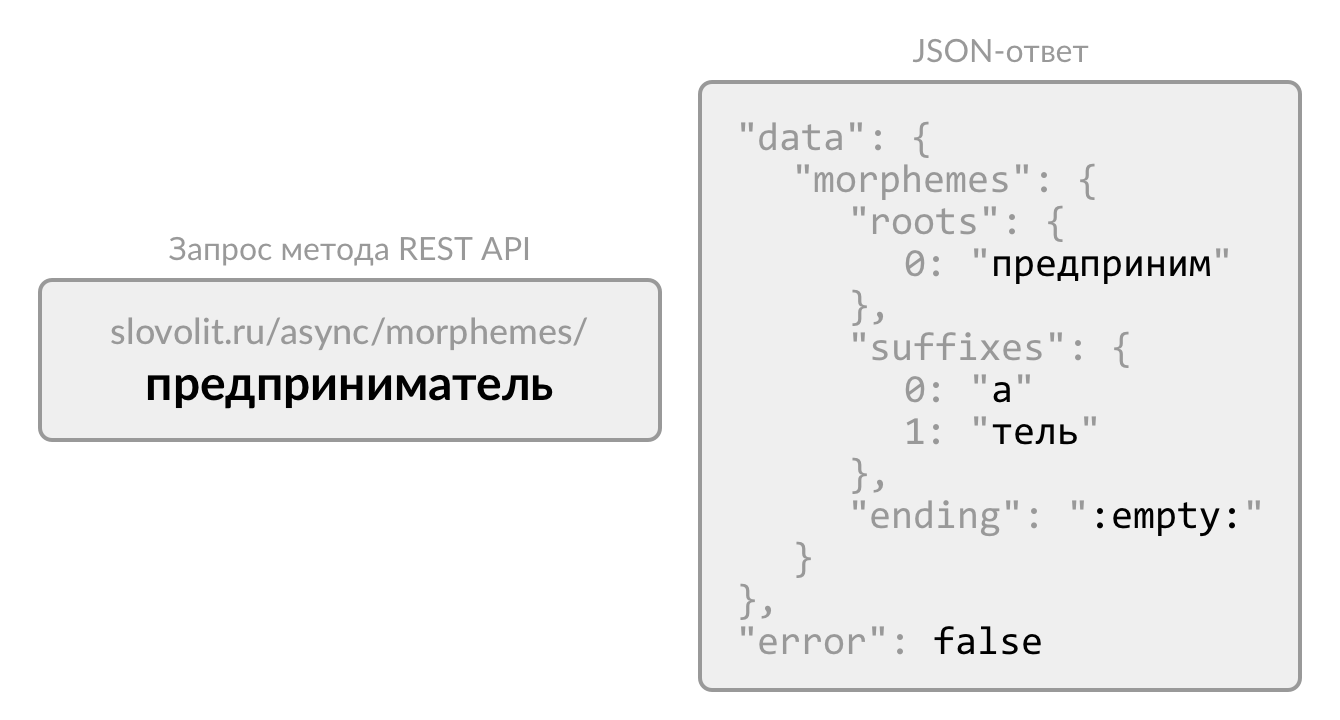
\includegraphics[scale=0.3]{api_method_example}
\caption{Пример ответа API-метода для морфемного анализа слова «предприниматель»}
\label{fig:api_method_example}
\end{figure}

На рисунке опущена строчка в JSON, отвечающая за специфичный код для библиотеки Morfana, которая строит графические обозначения морфем в интерфейсе.

Веб-сервис использует фреймворк Laravel. Он написан по схеме проектирования приложений MVC — Model-View-Controller (Рис. \ref{fig:mvc_architecture}). Схема обеспечивает разделение бизнес-логики, интерфейса и модели данных приложения.

\begin{figure}[ht!]
\centering
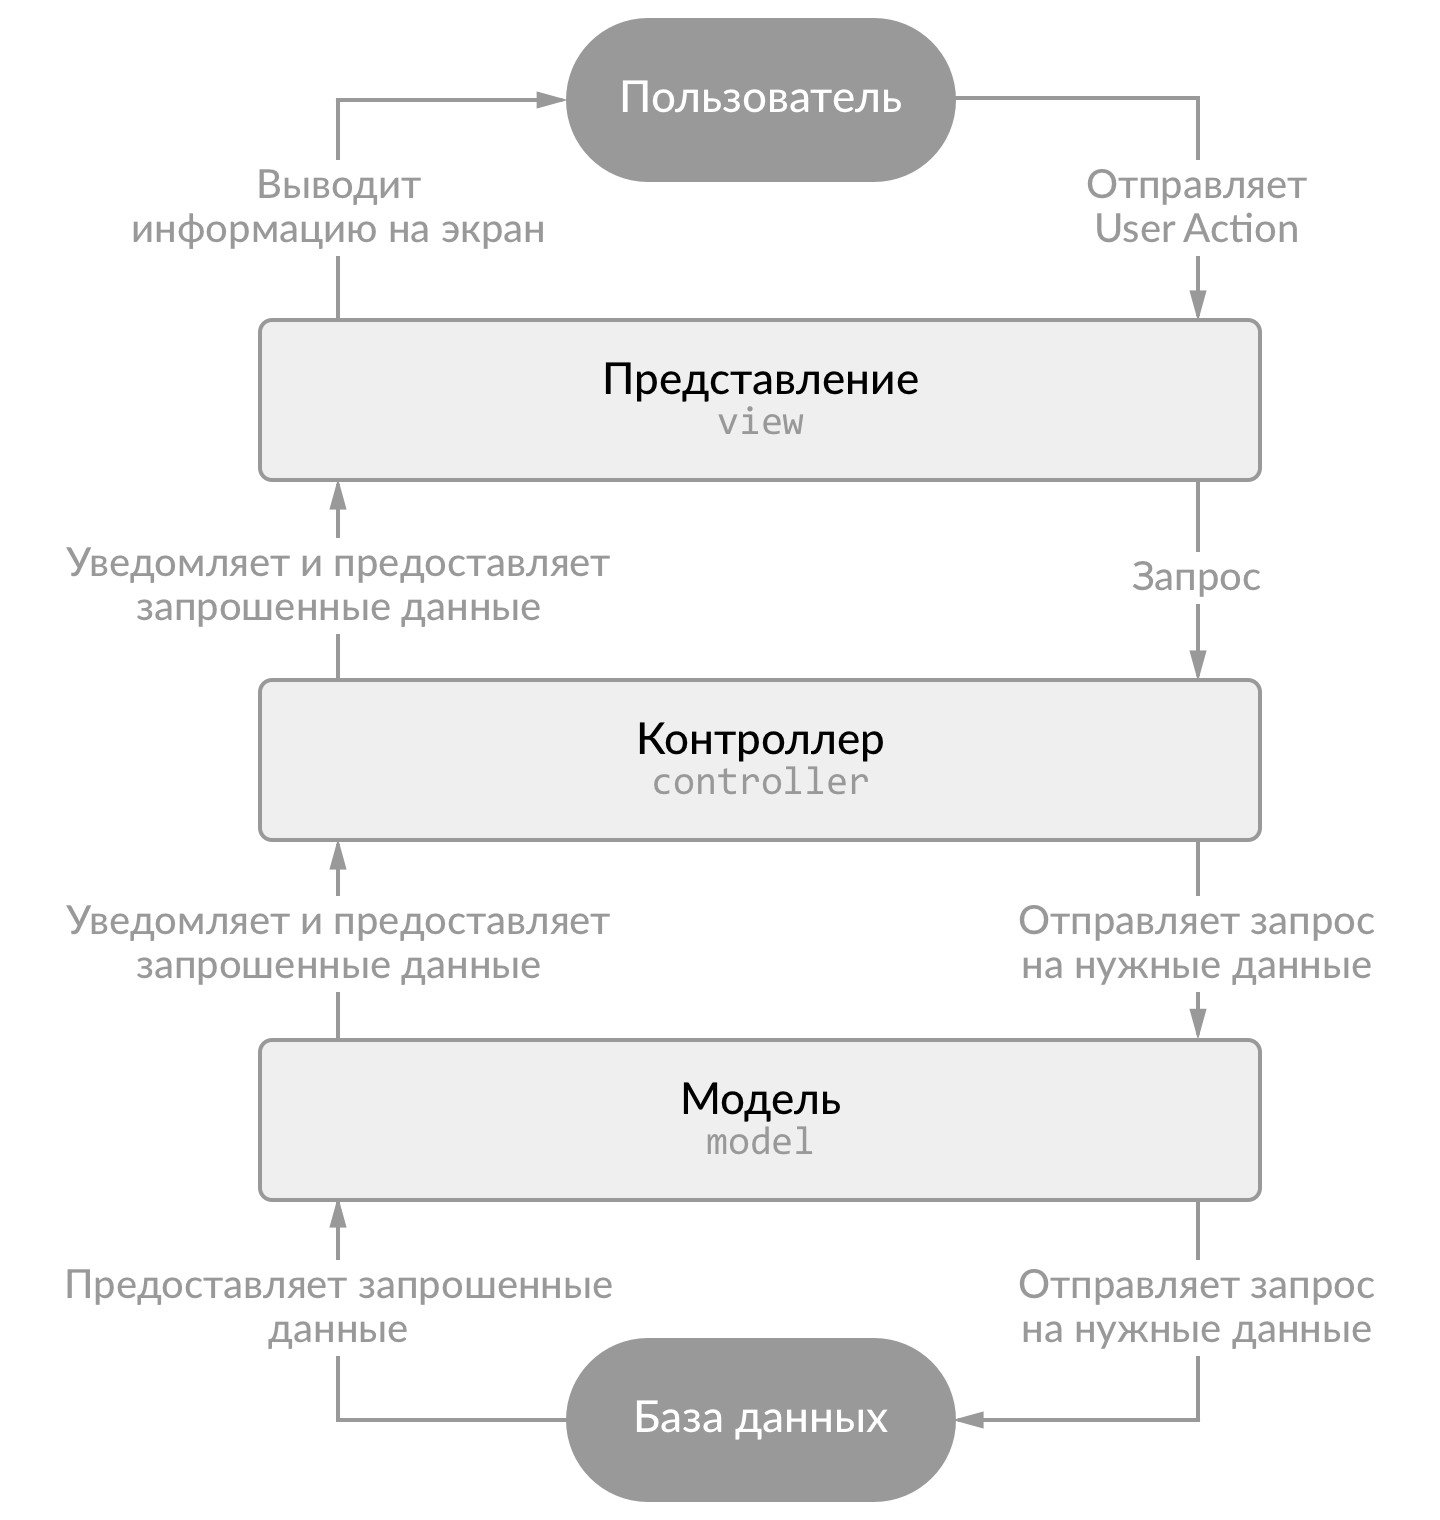
\includegraphics[scale=0.3]{mvc_architecture}
\caption{Серверная архитектура веб-приложения на фреймворке Laravel}
\label{fig:mvc_architecture}
\end{figure}

\section{Реализация веб-приложения}
Любой веб-сервис состоит из двух компонентов: интерфейс и серверная часть \cite{guide_web}. По запросу пользователя какой-либо страницы веб-сайта, сервер запускает необходимые процессы бизнес-логики, получает данные и генерирует HTML-страницу, которая вместе с CSS-стилями отдается браузеру клиента. Браузер же отрисовывает эту страницу на экране.

Для упрощения верстки стилей CSS, которые и задают вид всех элементов сайта, созданы препроцессоры, которые добавляют в синтаксис CSS переменные, условные операторы, а также функции и многое другое. Подробнее о сравнении некоторых препроцессоров можно прочитать в \cite{css_comparison}, а посмотреть репозитории самых популярных на Github \cite{github_css}. Для данного проекта был выбран препроцессор Sass \cite{sass}, с синтаксисом SCSS, который компилируется с помощью библиотеки для языка программирования Ruby.

Серверных же языков программирования существует множество: Python, Ruby, PHP, NodeJS, Go и другие. Для решения поставленной задачи был выбран язык программирования PHP, как один из самых популярных, не смотря на споры \cite{quora_1} и \cite{quora_2} о перспективах PHP. Причиной выбора языка также послужил используемый в работе фреймворк Laravel \cite{laravel}, написанный на языке PHP.

Все разборы разделены по компонентам, для отделения алгоритмов анализа слов от остальной бизнес-логики, отвечающей, например, за выполнение составной команды поиска.

\begin{itemize}
\item \textbf{Морфемный анализ}  \texttt{/async/morphemes/\{word\}} \\ Так как алгоритм реализован с нуля, исходя из потребностей системы, ему посвящена следующая глава этой статьи.
\item \textbf{Морфологический анализ}  \texttt{/async/morph/\{word\}} \\ Слово разбирается библиотекой \cite{phpmorphy}, затем заменяются аббревиатуры граммем на их расшифровки. Например, КР\_ПРИЛ — краткое прилагательное. К выдаче добавляется начальная форма слова.
\item \textbf{Подбор синонимов}  \texttt{/async/synonyms/\{word\}} \\ Происходит поиск начальной форма слова из \cite{phpmorphy} в словаре Абрамова \cite{dicts}. Формируется выдача.
\item \textbf{Значение слова}  \texttt{/async/meaning/\{word\}} \\ Как и при подборе синонимов, происходит поиск начальной форма слова из \cite{phpmorphy} в словаре Ожегова \cite{dicts}. Формируется выдача.
\end{itemize}

Использование веб-стека переносит нагрузку на сторону сервера, что уменьшает требовательность приложения к ресурсам аппаратной платформы. Также, исчезает проблема обновлений программы, так как используется всегда свежая версия.

\section{Алгоритм морфемного анализа}
Морфемный анализ не так популярен среди исследователей, так как имеет небольшую практическую применимость, поэтому было принято решение разработать собственный алгоритм получения структуры слова. Подробно алгоритм описан в материалах конференции «МСИТ 2016» \cite{msit}.

Алгоритм построен на последовательном переборе уже известных морфем в данном слове. Для этого был использован оцифрованный Морфемно-орфографическии словарь русского языка А. Н. Тихонова \cite{dicts}, в котором размечен большой объем слов, но сами типы морфем не обозначены. Второй словарь — морфемы в формате JSON из словаря Т. Ф. Ефремовой \cite{morph}, и данных сайта «Словород» \cite{slovorod}. Схема алгоритма представлена на Рис. \ref{fig:algo_scheme}.

\begin{figure}[ht!]
\centering
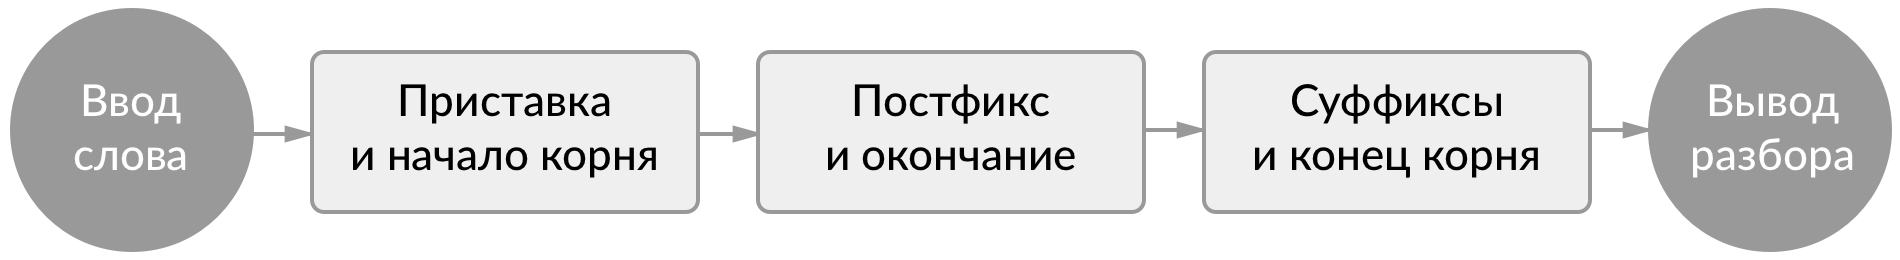
\includegraphics[scale=0.26]{algo_scheme}
\caption{Упрощенная схема действия алгоритма морфемного анализа}
\label{fig:algo_scheme}
\end{figure}

Записи в словаре Тихонова выглядят как слово, разделенного слешами. Например, для слова частнопредпринимательский — \textbf{частн/о/предприним/а'/тель/ск/ий} система производит поиск по словарю и получает строчку такого вида. Далее алгоритм, используя преобразование строчки в массив с помощью функции explode получает массив морфем, но каких именно, неизвестно. С помощью данных морфемного словаря и последовательной проверки каждого элемента массива получается результирующий массив, который в дальнейшем используется API-методом для выдачи другим контроллерам системы. 

Представленный алгоритм обладает ограничением: достоверно определить корень не всегда получается, так как полного словаря корней не существует. На данный момент существует и обновляется корнеслов Федора Шимкевича \cite{slovorod} на сайте «Словород», но он не является полным. В алгоритме же проблема обходится путем отметки начала и конца предполагаемого корневого массива (Рис. \ref{fig:root_array}).

\begin{figure}[ht!]
\centering
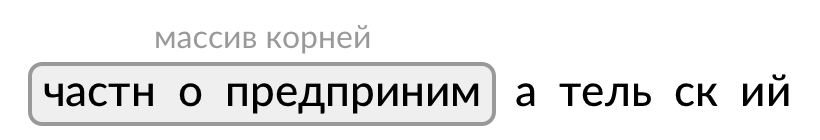
\includegraphics[scale=0.32]{root_array}
\caption{Выделенный массив корней}
\label{fig:root_array}
\end{figure}

Данный метод не работает в случаях, когда слово сложное (т. е. имеет несколько корней) и написано через дефис. В данном случае целесообразнее предварительно разбивать слово на несколько частей, а затем разбирать эти части.

\section{Графический интерфейс}
Тренды в дизайне интерфейсов уже давно перешли от скевоморфизма к простым формам и так называемому «плоскому» дизайну. Приложения избавляются от лишних деталей, чтобы перенести информацию во главу угла, тем самым повышая получаемую пользу.

Во время проектирования интерфейса данного сервиса применен подход «mobile-first», что позволило улучшить пользовательский опыт на мобильных устройствах. Это подход, при котором проектирование сервиса начинается с мобильной версии, а не с версии для больших экранов, как это делается повсеместно. Подробнее об этом подходе написано в книге \cite{mobile_first}.

Дизайн выдачи результатов вдохновлен сервисом Wolfram Alpha, который акцентирует внимание на полезной информации. Интерфейс сервиса в двух разрешениях показан на Рис. \ref{fig:interface}.

\begin{figure}[ht!]
\centering
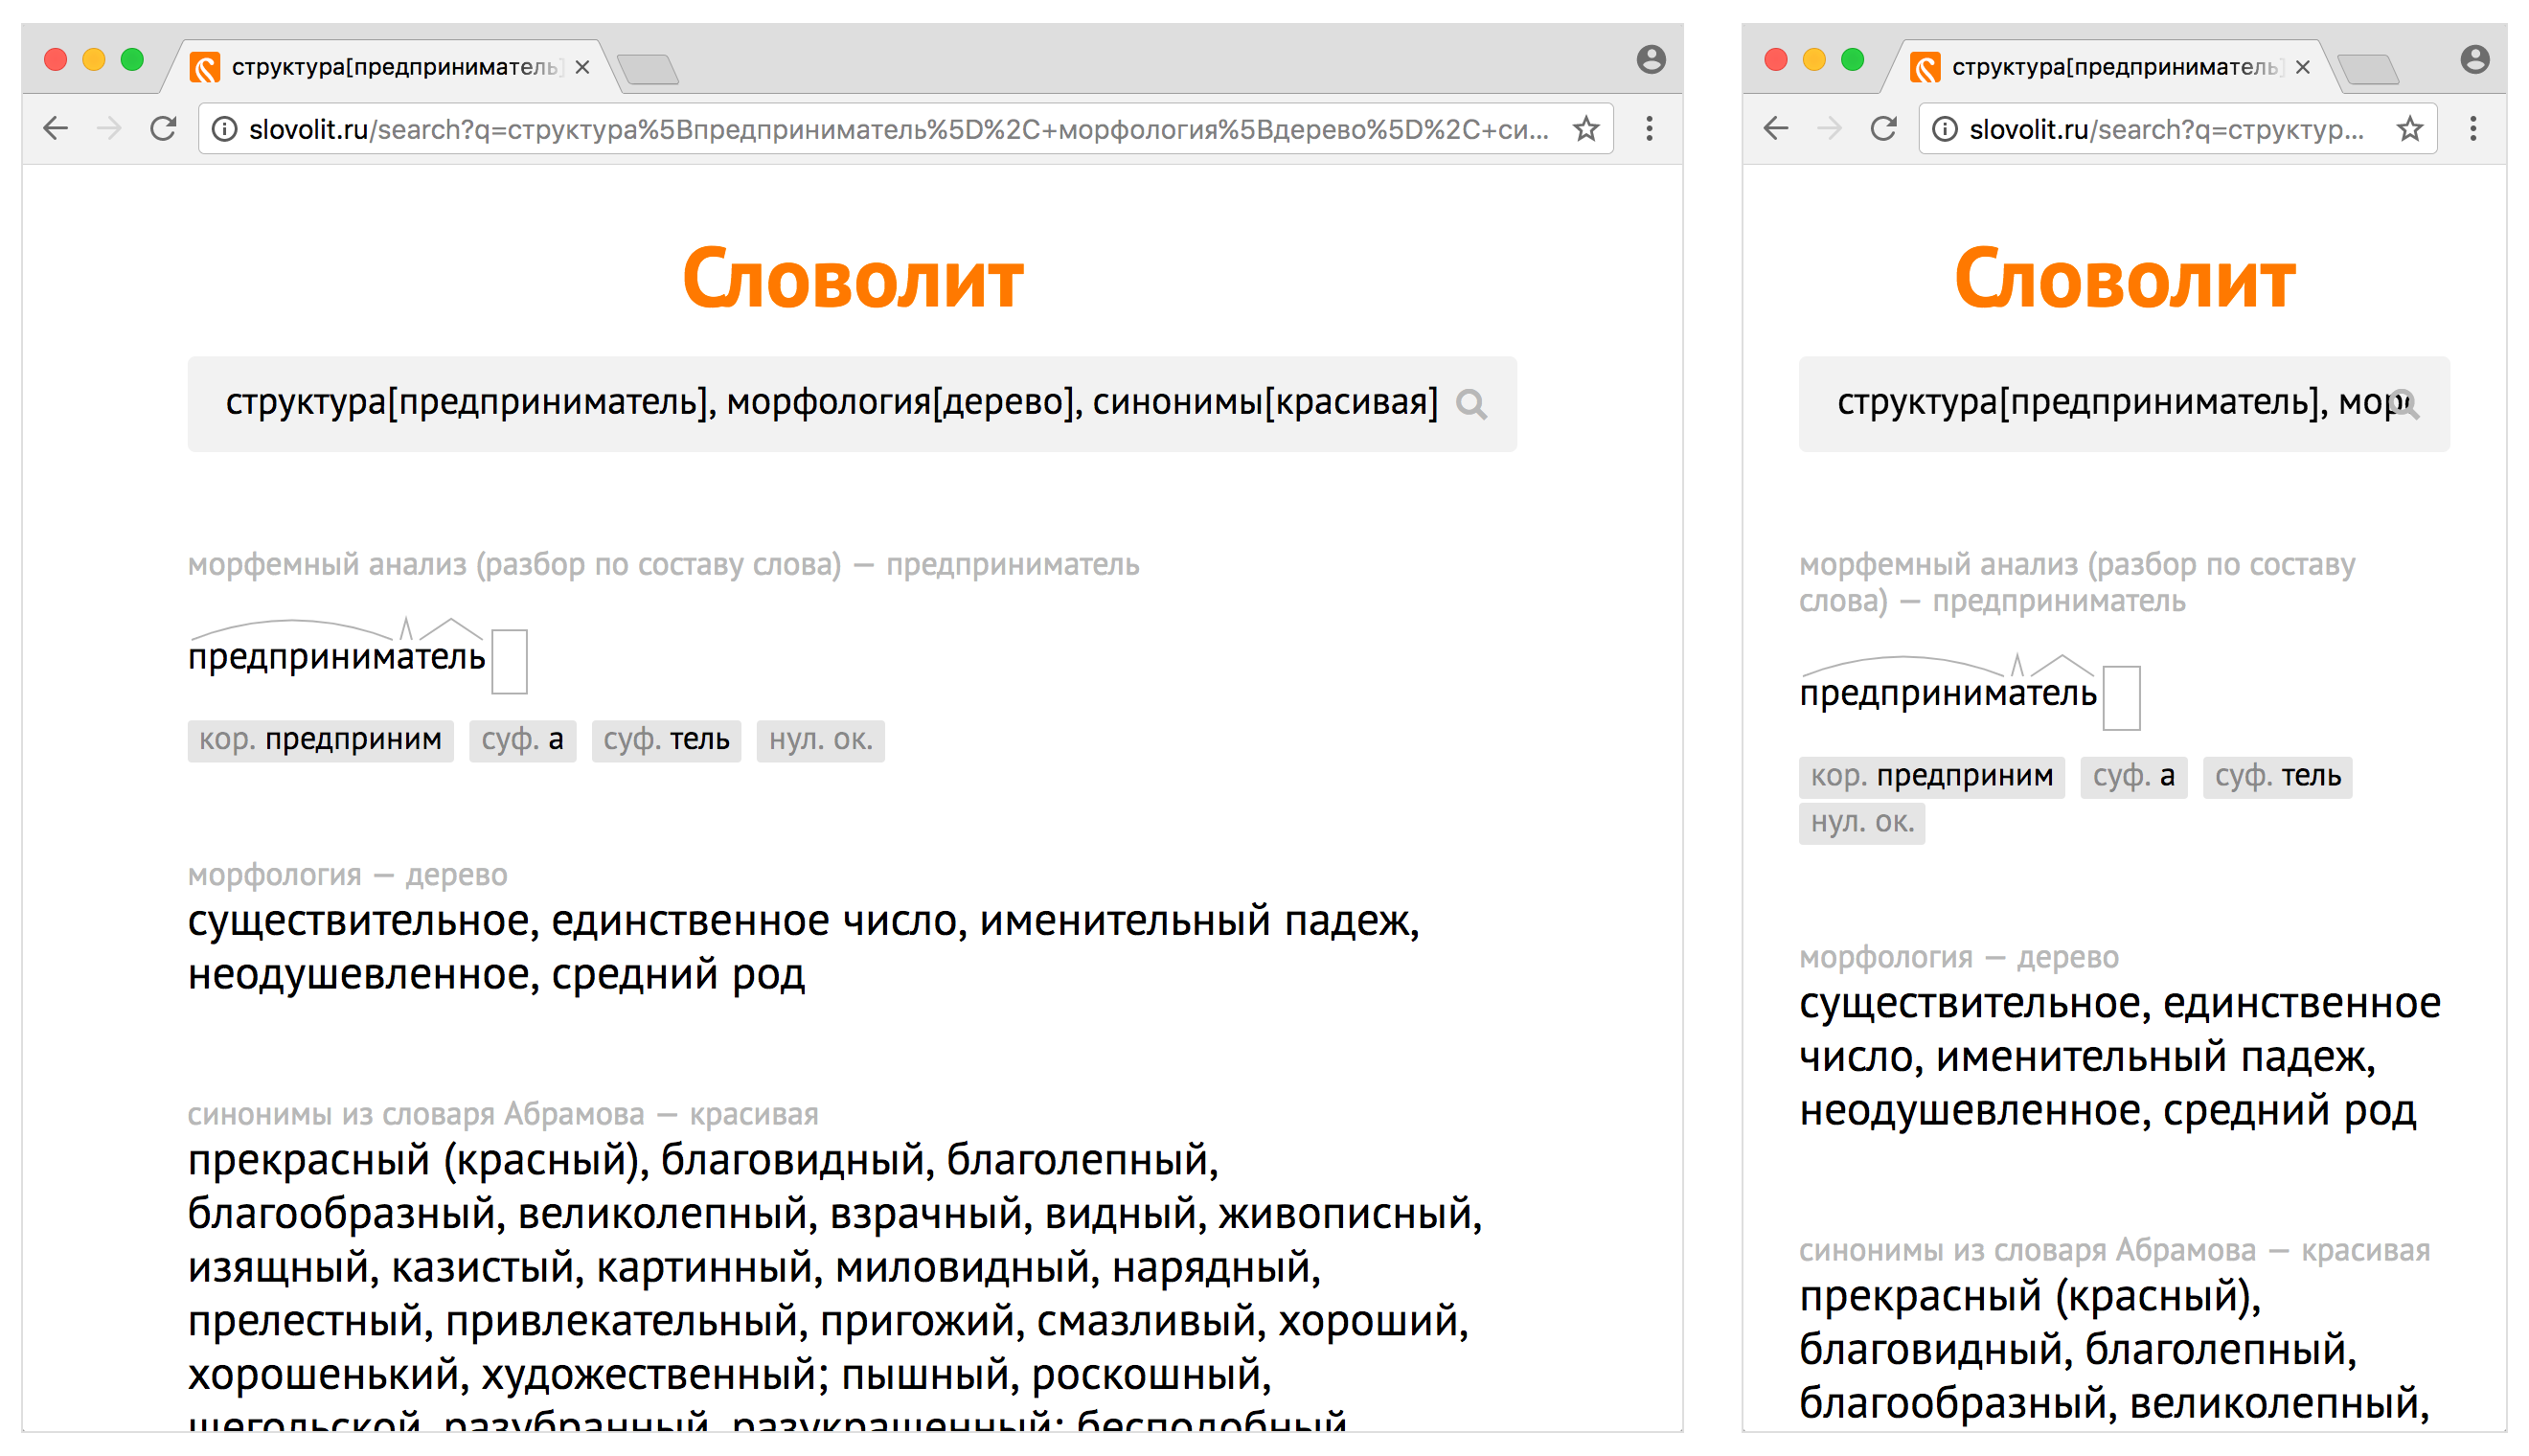
\includegraphics[scale=0.18]{interface}
\caption{Интерфейс веб-сервиса: в настольном и мобильном браузере}
\label{fig:interface}
\end{figure}

\section{Нерешенные проблемы}
Представленный в работе алгоритм морфемного разбора имеют существенное ограничение, связанное с отсутствием слова в словаре Тихонова. Так как язык постоянно расширяется, трудоемко иметь свежий словарь, покрытие разбираемых слов будет постепенно уменьшаться.

Другая проблема состоит в том, что алгоритм не может с максимальной точностью определить корень, потому что словаря корней также не существует, что следует из постоянного расширения языка.

Эти проблемы можно решить разработкой платформы, которая будет собирать данные о словах из различных источников, например, блогов, новостных сервисов или открытых корпусов. Путем частотного анализа и частичного разбора этих слов можно выявлять новые корни и пополнять словарь.

\section*{Заключение}
Разработанный веб-сервис позволяет производить различные анализы слов, а также комбинировать результаты посредством использования различных команд в строке запросов. Сервис реализован в виде адаптивного веб-сайта, что позволяет использовать его как на настольных, так и на мобильных устройствах.

Разработанный алгоритм морфемного анализа может помочь другим специалистам при разработке текстовых анализаторов, например, для выявления суффиксов.

Представленный в данной статье веб-сервис, в отличие от других сервисов в сфере автоматической обработки слов, позволяет разбирать несколько слов одновременно, а также комбинировать результаты работы сервиса для разных слов на одной странице браузера.

В будущем планируется добавить алгоритм «предсказания» слов, которых нет в словаре, а также добавить в сервис фонетический и другие разборы. Кроме того, планируется разработка открытого АПИ для сторонних разработчиков для удобного пользования сервисом.

%%\newpage

\printbibliography[title={Список использованных источников}]

\end{document}
